%\VignetteIndexEntry{An Introduction to the BUMHMM pipeline}
%\VignetteKeywords{BUMHMM, structure probing, RNA}
%\VignettePackage{BUMHMM}
%\VignetteEngine{knitr::knitr}

\documentclass{article}\usepackage[]{graphicx}\usepackage[usenames,dvipsnames]{color}
%% maxwidth is the original width if it is less than linewidth
%% otherwise use linewidth (to make sure the graphics do not exceed the margin)
\makeatletter
\def\maxwidth{ %
  \ifdim\Gin@nat@width>\linewidth
    \linewidth
  \else
    \Gin@nat@width
  \fi
}
\makeatother

\definecolor{fgcolor}{rgb}{0.345, 0.345, 0.345}
\newcommand{\hlnum}[1]{\textcolor[rgb]{0.686,0.059,0.569}{#1}}%
\newcommand{\hlstr}[1]{\textcolor[rgb]{0.192,0.494,0.8}{#1}}%
\newcommand{\hlcom}[1]{\textcolor[rgb]{0.678,0.584,0.686}{\textit{#1}}}%
\newcommand{\hlopt}[1]{\textcolor[rgb]{0,0,0}{#1}}%
\newcommand{\hlstd}[1]{\textcolor[rgb]{0.345,0.345,0.345}{#1}}%
\newcommand{\hlkwa}[1]{\textcolor[rgb]{0.161,0.373,0.58}{\textbf{#1}}}%
\newcommand{\hlkwb}[1]{\textcolor[rgb]{0.69,0.353,0.396}{#1}}%
\newcommand{\hlkwc}[1]{\textcolor[rgb]{0.333,0.667,0.333}{#1}}%
\newcommand{\hlkwd}[1]{\textcolor[rgb]{0.737,0.353,0.396}{\textbf{#1}}}%
\let\hlipl\hlkwb

\usepackage{framed}
\makeatletter
\newenvironment{kframe}{%
 \def\at@end@of@kframe{}%
 \ifinner\ifhmode%
  \def\at@end@of@kframe{\end{minipage}}%
  \begin{minipage}{\columnwidth}%
 \fi\fi%
 \def\FrameCommand##1{\hskip\@totalleftmargin \hskip-\fboxsep
 \colorbox{shadecolor}{##1}\hskip-\fboxsep
     % There is no \\@totalrightmargin, so:
     \hskip-\linewidth \hskip-\@totalleftmargin \hskip\columnwidth}%
 \MakeFramed {\advance\hsize-\width
   \@totalleftmargin\z@ \linewidth\hsize
   \@setminipage}}%
 {\par\unskip\endMakeFramed%
 \at@end@of@kframe}
\makeatother

\definecolor{shadecolor}{rgb}{.97, .97, .97}
\definecolor{messagecolor}{rgb}{0, 0, 0}
\definecolor{warningcolor}{rgb}{1, 0, 1}
\definecolor{errorcolor}{rgb}{1, 0, 0}
\newenvironment{knitrout}{}{} % an empty environment to be redefined in TeX

\usepackage{alltt}

\RequirePackage{/home/aselega/R/x86_64-pc-linux-gnu-library/3.3/BiocStyle/resources/tex/Bioconductor}

\AtBeginDocument{\bibliographystyle{/home/aselega/R/x86_64-pc-linux-gnu-library/3.3/BiocStyle/resources/tex/unsrturl}}


\bioctitle[BUMHMM: Computational pipeline for modelling structure probing data]{BUMHMM: Probabilistic computational pipeline for modelling RNA structure probing data}
\author{Alina Selega\footnote{alina.selega@ed.ac.uk or alina.selega@gmail.com}}
\date{Modified: October 25, 2016. Compiled: \today}
\IfFileExists{upquote.sty}{\usepackage{upquote}}{}
\begin{document}

\maketitle

\tableofcontents

\section{Introduction}

RNA structure is known to be a key regulator of many important mechanisms, such
as RNA stability, transcription, and mRNA translation. RNA structural regulatory
elements are interrogated with chemical and enzymatic structure probing
\cite{kubota2015progress}. In these experiments, a chemical agent reacts with
the RNA molecule in a structure-dependent way, cleaving or otherwise modifying
its flexible parts. These modified positions can then be detected, providing
valuable structural information that can be used for structure prediction
\cite{wu2015improved}.

Specifically, chemical modification terminates the reverse transcription
reaction, resulting in the reverse transcriptase (RT) dropping off at the
modified positions. These positions of drop-off can be then mapped back to the
reference sequence. However, the challenge lies in the stochasticity of this
process as the RT can also drop off randomly. To address this, a complementary
control experiment is routinely performed to monitor random RT drop-offs when no
reagent is used.

Let us consider a toy example of data obtained in a paired-end sequencing
structure probing experiment (Fig. 1). We'll focus on a particular nucleotide G
and analyse the data from a control experiment (with no reagent added) and a
treatment experiment (with RNAs modified by the reagent). In control conditions,
we mapped 5 fragments overlapping with the nucleotide G, one of which also
terminated at that position. Thus, this nucleotide had a coverage of 5 and a
drop-off count of 1 (the number of times the RT dropped off immediately after
this position), giving it a \textit{drop-off rate} of \( \frac{1}{5} \)
(formally defined below). In treatment conditions, more fragments terminated at
this position and we measured a drop-off rate of \( \frac{4}{5} \). This seems
to suggest that the next nucleotide T has been modified by the reagent and
perhaps corresponds to a flexible site within the molecule. However, would our
conclusion remain the same had we observed a higher drop-off rate in control
conditions to start with? In fact, how high would this control drop-off rate
have to be for us to dismiss the drop-off rate of \( \frac{4}{5} \) as a noisy
measurement of randrom drop-off rather than an indication of real modification?

\begin{figure}[h]
\caption{Toy example of structure probing data.}
\centering
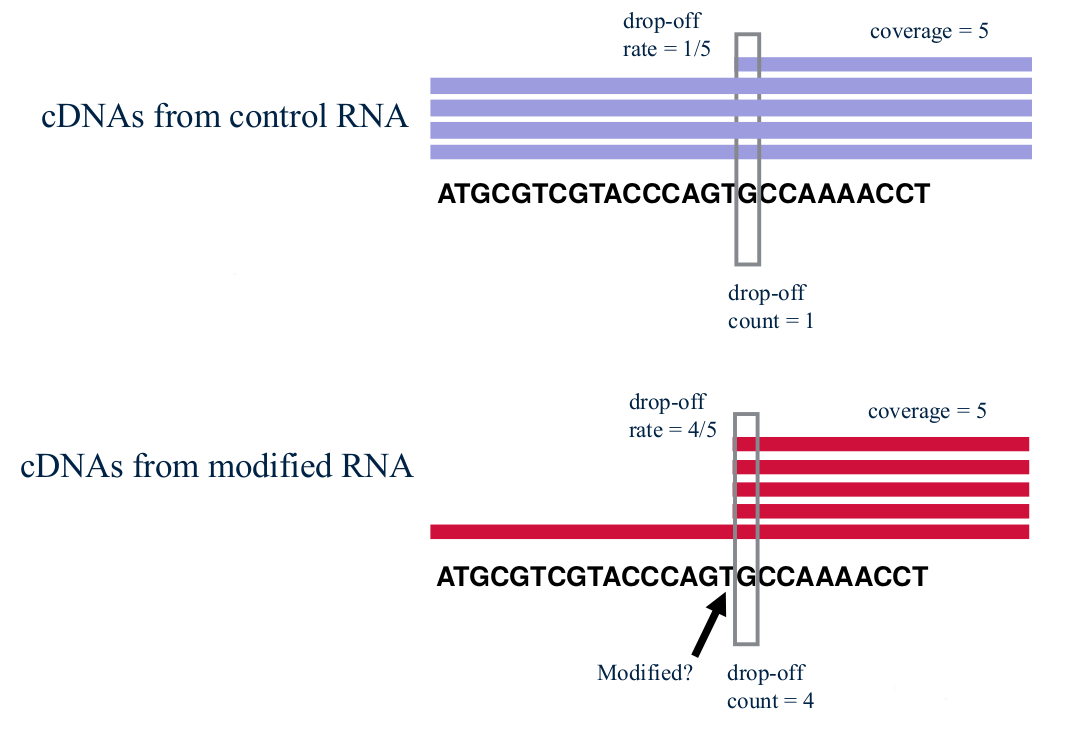
\includegraphics[width=0.9\textwidth]{toyEx_structureProbing.png}
\end{figure}

This question reinforces the need for deciding statistically whether the
drop-off rate in treatment conditions is significantly higher than the drop-off
rate in control. To do this, we must understand how much noise can be expected
in control conditions. If the treatment drop-off rate is outside of this range
of drop-off rate variability, then we could deem it as significantly higher.

We developed Beta-Uniform Mixture hidden Markov model (\verb|BUM-HMM|)
\cite{selega2016robust}, a statistical framework for modelling reactivity scores
from an RNA structure probing experiment such as SHAPE
\cite{spitale2013rna} or ChemModSeq \cite{hector2014snapshots}. \verb|BUM-HMM|
implements the intuition outlined above by utilising data from multiple
experimental replicates and quantifying the variability of the RT drop-offs.
\verb|BUM-HMM| also provides empirical strategies to correct intrinsic biases in
the data. It generates a probabilistic output measuring the probability of
modification for each nucleotide transcriptome-wide.

The \verb|BUMHMM| package implements the functionality of the \verb|BUM-HMM|
model. This vignette provides an example workflow for using the \verb|BUMHMM|
package on the structure probing data set for the yeast ribosomal RNA 18S,
obtained in an experiment with random priming and paired-end sequencing
(available in the Gene Expression Omnibus under accession number GSE52878).

\section{Data format}

The \verb|BUMHMM| pipeline requires three data sets for all nucleotide
positions:

\begin{itemize}
\item the coverage (or the number of reads overlapping with this position),
\item the drop-off count (or the number of times the RT dropped off at the next
    nucleotide),
\item and the drop-off rate at this position.
\end{itemize}

The coverage and the drop-off counts are the data obtained in a structure
probing experiment with paired-end sequencing. The drop-off rate $r$ at each
nucleotide position is computed as the ratio between its drop-off count $k$ and
the coverage $n$: \(r = \frac{k}{n} \). Such data sets can be easily stored in a
\Biocpkg{SummarizedExperiment} object, commonly used to represent data from
sequencing-based experiments such as RNA-Seq.

The key strength of \verb|BUMHMM| is accounting for the biological
variability of the data and thus, it requires data sets available in multiple
replicates. The data set \texttt{se} provided with this package (accession
number GSE52878) is available in triplicates and was obtained in a structure
probing experiment on the 18S ribosomal RNA using the DMS chemical probing agent
\cite{wells200032}.

\begin{knitrout}
\definecolor{shadecolor}{rgb}{0.969, 0.969, 0.969}\color{fgcolor}\begin{kframe}
\begin{alltt}
\hlkwd{suppressPackageStartupMessages}\hlstd{(\{}
    \hlkwd{library}\hlstd{(BUMHMM)}
    \hlkwd{library}\hlstd{(Biostrings)}
    \hlkwd{library}\hlstd{(SummarizedExperiment)}
\hlstd{\})}
\hlstd{se}
\end{alltt}
\begin{verbatim}
## class: SummarizedExperiment 
## dim: 1800 6 
## metadata(0):
## assays(3): coverage dropoff_count dropoff_rate
## rownames: NULL
## rowData names(1): nucl
## colnames(6): C1 C2 ... T2 T3
## colData names(1): replicate
\end{verbatim}
\end{kframe}
\end{knitrout}

We see that 18S has 1,800 nucleotides (represented as rows in \texttt{se}) and
that the data set has 6 replicates: 3 control experiments followed by 3
treatment experiments (represented as columns in \texttt{se}). The assays
correspond to different data sets, namely, the coverage, drop-off count, and
drop-off rate information for each nucleotide. One could quickly access the
coverage information for control experimental replicates (labelled 'C1', 'C2',
'C3') as follows:

\begin{knitrout}
\definecolor{shadecolor}{rgb}{0.969, 0.969, 0.969}\color{fgcolor}\begin{kframe}
\begin{alltt}
\hlstd{controls} \hlkwb{<-} \hlstd{se[, se}\hlopt{$}\hlstd{replicate} \hlopt{==} \hlstr{"control"}\hlstd{]}
\hlkwd{head}\hlstd{(}\hlkwd{assay}\hlstd{(controls,} \hlstr{'coverage'}\hlstd{))}
\end{alltt}
\begin{verbatim}
##          C1     C2     C3
## [1,] 382943 276113 135209
## [2,] 399211 280523 137706
## [3,] 403519 284622 140211
## [4,] 404242 287589 144656
## [5,] 404463 288348 147167
## [6,] 404506 288445 147687
\end{verbatim}
\end{kframe}
\end{knitrout}

We also provide the associated genomic sequence of 18S, accessible through the
\Rfunction{rowData} function which stores information about the rows, in this
case corresponding to the nucleobases:

\begin{knitrout}
\definecolor{shadecolor}{rgb}{0.969, 0.969, 0.969}\color{fgcolor}\begin{kframe}
\begin{alltt}
\hlkwd{rowData}\hlstd{(controls)[}\hlnum{1}\hlopt{:}\hlnum{4}\hlstd{,]}
\end{alltt}
\begin{verbatim}
##   Views on a 1800-letter DNAString subject
## subject: TATCTGGTTGATCCTGCCAGTAGTCATATGCTTGTCTCA...AACAAGGTTTCCGTAGGTGAACCTGCGGAAGGATCATTA
## views:
##     start end width
## [1]     1   1     1 [T]
## [2]     2   2     1 [A]
## [3]     3   3     1 [T]
## [4]     4   4     1 [C]
\end{verbatim}
\end{kframe}
\end{knitrout}

Similarly, the function \Rfunction{colData} stores the description of the
columns, which correspond to the experimental replicates:

\begin{knitrout}
\definecolor{shadecolor}{rgb}{0.969, 0.969, 0.969}\color{fgcolor}\begin{kframe}
\begin{alltt}
\hlkwd{colData}\hlstd{(controls)}
\end{alltt}
\begin{verbatim}
## DataFrame with 3 rows and 1 column
##      replicate
##    <character>
## C1     control
## C2     control
## C3     control
\end{verbatim}
\end{kframe}
\end{knitrout}

For transcriptome-wide experiments, the data over different chromosomes should
be concatenated row-wise.

To briefly illustrate the data set, let us examine the 300th nucleotide:

\begin{knitrout}
\definecolor{shadecolor}{rgb}{0.969, 0.969, 0.969}\color{fgcolor}\begin{kframe}
\begin{alltt}
\hlstd{pos} \hlkwb{<-} \hlnum{300}
\hlkwd{assay}\hlstd{(controls,} \hlstr{'coverage'}\hlstd{)[pos,} \hlnum{1}\hlstd{]}
\end{alltt}
\begin{verbatim}
##     C1 
## 813073
\end{verbatim}
\begin{alltt}
\hlkwd{assay}\hlstd{(controls,} \hlstr{'dropoff_count'}\hlstd{)[pos,} \hlnum{1}\hlstd{]}
\end{alltt}
\begin{verbatim}
##   C1 
## 1837
\end{verbatim}
\begin{alltt}
\hlkwd{assay}\hlstd{(controls,} \hlstr{'dropoff_rate'}\hlstd{)[pos,} \hlnum{1}\hlstd{]}
\end{alltt}
\begin{verbatim}
##         C1 
## 0.00225933
\end{verbatim}
\end{kframe}
\end{knitrout}

We see that it had coverage of 813073
in the first control experimental replicate, of which the reverse transcription
randomly terminated at that position
1837 times, giving it a drop-off
rate of 0.00226.

\begin{knitrout}
\definecolor{shadecolor}{rgb}{0.969, 0.969, 0.969}\color{fgcolor}\begin{kframe}
\begin{alltt}
\hlstd{treatments} \hlkwb{<-} \hlstd{se[, se}\hlopt{$}\hlstd{replicate} \hlopt{==} \hlstr{"treatment"}\hlstd{]}
\hlkwd{assay}\hlstd{(treatments,} \hlstr{'coverage'}\hlstd{)[pos,} \hlnum{1}\hlstd{]}
\end{alltt}
\begin{verbatim}
##      T1 
## 1640501
\end{verbatim}
\begin{alltt}
\hlkwd{assay}\hlstd{(treatments,} \hlstr{'dropoff_count'}\hlstd{)[pos,} \hlnum{1}\hlstd{]}
\end{alltt}
\begin{verbatim}
##   T1 
## 4844
\end{verbatim}
\begin{alltt}
\hlkwd{assay}\hlstd{(treatments,} \hlstr{'dropoff_rate'}\hlstd{)[pos,} \hlnum{1}\hlstd{]}
\end{alltt}
\begin{verbatim}
##          T1 
## 0.002952757
\end{verbatim}
\end{kframe}
\end{knitrout}

In the presence of a chemical probe (in the first treatment replicate), the
coverage and drop-off count at that position were higher but the drop-off rate
remained roughly similar,
0.00295.

\section{The overview of pipeline}

The logic of structure probing experiments associates the binding accessibility
of a nucleotide with its structural flexibility, i.e. double-stranded
nucleotides or those otherwise protected (e.g. by a protein interaction) will
not be available for interaction with the chemical reagent. In contrast, those
nucleotides located in flexible parts of the molecule, could be chemically
modified by the reagent and will therefore correspond to the positions at which
the RT drops off. Thus, we expect the nucleotides immediately downstream from
the modification sites within the transcript to have a high drop-off rate in the
presence of a reagent; higher than what we observe in control conditions.

To quantify the variability in drop-off rate measured in control conditions,
\verb|BUMHMM| compares the drop-off rates at each nucleotide position between
two \textit{control} experimental replicates, ${C_i}$ and ${C_j}$:

\[log \Big( \frac{r_{C_i}}{r_{C_j}} \Big) \]

If the drop-off rates $r_{C_i}$ and $r_{C_j}$ are similar in a pair of control
replicates, the above log-ratio will be close to 0, indicating little
to no variability in drop-off rate. In contrast, different drop-off rates will
result in a large log-ratio (in absolute value). Computing these per-nucleotide
log-ratios for all pairs of control experimental replicates defines a
\textit{null distribution}, which quantifies how much variability in drop-off
rate we can observe between two experimental replicates simply by chance, in the
absence of any reagent. (Note that due to a log transform, the drop-off rates
$r = 0$ are not allowed.)

We now compute this log-ratio between the drop-off rates in all pairs of
\textit{treatment} and \textit{control} experimental replicates, ${T_i}$ and
${C_j}$:

\[log \Big( \frac{r_{T_i}}{r_{C_j}} \Big) \]

We expect the neighbour of a modified nucleotide to have a much larger drop-off
rate in a treatment experiment compared to control conditions, generating a
large log-ratio for this pair of experimental replicates. By comparing each
treatment-control log-ratio to the null distribution, we can find those
nucleotide positions that demonstrate differences in drop-off rate larger than
what can be expected by chance.

The next section goes through the steps of the \verb|BUMHMM| pipeline using the
provided data set \texttt{se} as an example.

\section{BUMHMM pipeline steps}

\subsection{Selecting pairs of nucleotides}

We first need to select nucleotide positions in each experimental replicate for
which we will compute the log-ratios. This is implemented with the function
\Rfunction{selectNuclPos}. This function requires the coverage and drop-off
count information stored in \texttt{se}, the numbers of control and treatment
experimental replicates (\texttt{Nc} and \texttt{Nt}, correspondingly), and a
user-specified coverage threshold \texttt{t}. Nucleotides with coverage $n < t$
will not be considered.

In our data set, we have 3 control and 3 treatment replicates, so if we set the
minimum allowed coverage as $t = 1$, we can make the following function call:

\begin{knitrout}
\definecolor{shadecolor}{rgb}{0.969, 0.969, 0.969}\color{fgcolor}\begin{kframe}
\begin{alltt}
\hlstd{Nc} \hlkwb{<-} \hlstd{Nt} \hlkwb{<-} \hlnum{3}
\hlstd{t} \hlkwb{<-} \hlnum{1}
\hlstd{nuclSelection} \hlkwb{<-} \hlkwd{selectNuclPos}\hlstd{(se, Nc, Nt, t)}
\hlkwd{List}\hlstd{(nuclSelection)}
\end{alltt}
\begin{verbatim}
## List of length 2
## names(2): analysedC analysedCT
\end{verbatim}
\end{kframe}
\end{knitrout}

The function \Rfunction{selectNuclPos} returns a list with two elements:

\begin{itemize}

  \item \texttt{analysedC} is a list where each element corresponds to a
  control-control replicate comparison. Each element holds indices of
  nucleotides that have coverage $n >= t$ and a drop-off count $k > 0$ in both
  replicates of that comparison. Thus, each element stores those nucleotide
  positions for which we can compute the log-ratio for the corresponding pair of
  control replicates.

  \item \texttt{analysedCT} is a list where each element corresponds to a
  treatment-control replicate comparison. Again, each element holds indices of
  nucleotides that have coverage $n >= t$ and a drop-off count $k > 0$ in both
  replicates of that comparison.

\end{itemize}

The pairwise control replicate comparisons are enumerated with the function
\Rfunction{combn} from the \verb|utils| package:

\begin{knitrout}
\definecolor{shadecolor}{rgb}{0.969, 0.969, 0.969}\color{fgcolor}\begin{kframe}
\begin{alltt}
\hlkwd{t}\hlstd{(}\hlkwd{combn}\hlstd{(Nc,} \hlnum{2}\hlstd{))}
\end{alltt}
\begin{verbatim}
##      [,1] [,2]
## [1,]    1    2
## [2,]    1    3
## [3,]    2    3
\end{verbatim}
\end{kframe}
\end{knitrout}

Thus, the first element of \texttt{analysedC} corresponds to comparing the
control replicate 1 to control replicate 2. The comparisons between treatment
and control replicates are computed similarly.

\begin{knitrout}
\definecolor{shadecolor}{rgb}{0.969, 0.969, 0.969}\color{fgcolor}\begin{kframe}
\begin{alltt}
\hlkwd{length}\hlstd{(nuclSelection}\hlopt{$}\hlstd{analysedC[[}\hlnum{1}\hlstd{]])}
\end{alltt}
\begin{verbatim}
## [1] 1713
\end{verbatim}
\begin{alltt}
\hlkwd{length}\hlstd{(nuclSelection}\hlopt{$}\hlstd{analysedCT[[}\hlnum{1}\hlstd{]])}
\end{alltt}
\begin{verbatim}
## [1] 1723
\end{verbatim}
\end{kframe}
\end{knitrout}

We select 1713 nucleotide positions for
computing the log-ratios for the first control-control comparison and
1723 positions for the first
treatment-control comparison.

\subsection{Scaling the drop-off rates across replicates}

Because \verb|BUMHMM| works with data collected in multiple experimental
replicates, it is important to ensure that the drop-off rates do not differ
dramatically between replicates. Thus, the second step of the pipeline scales
the drop-off rates of nucleotides selected for pairwise comparisons to have a
common median value. This is implemented with a function \Rfunction{scaleDOR},
which requires the data container \texttt{se}, the output of the function
\Rfunction{selectNuclPos} (described above), and the numbers of replicates. It
returns the updated drop-off rates such that the selected positions have the
same median drop-off rate in all replicates:

\begin{knitrout}
\definecolor{shadecolor}{rgb}{0.969, 0.969, 0.969}\color{fgcolor}\begin{kframe}
\begin{alltt}
\hlcom{## Medians of original drop-off rates in each replicate}
\hlkwd{apply}\hlstd{(}\hlkwd{assay}\hlstd{(se,} \hlstr{'dropoff_rate'}\hlstd{),} \hlnum{2}\hlstd{, median)}
\end{alltt}
\begin{verbatim}
##          C1          C2          C3          T1          T2          T3 
## 0.001005071 0.001025182 0.003684315 0.001608314 0.001302076 0.003380141
\end{verbatim}
\begin{alltt}
\hlcom{## Scale drop-off rates}
\hlkwd{assay}\hlstd{(se,} \hlstr{"dropoff_rate"}\hlstd{)} \hlkwb{<-} \hlkwd{scaleDOR}\hlstd{(se, nuclSelection, Nc, Nt)}

\hlcom{## Medians of scaled drop-off rates in each replicate}
\hlkwd{apply}\hlstd{(}\hlkwd{assay}\hlstd{(se,} \hlstr{'dropoff_rate'}\hlstd{),} \hlnum{2}\hlstd{, median)}
\end{alltt}
\begin{verbatim}
##          C1          C2          C3          T1          T2          T3 
## 0.001618859 0.001611737 0.001707502 0.001641554 0.001708537 0.001719018
\end{verbatim}
\end{kframe}
\end{knitrout}

After scaling, medians are much more similar across replicates (they are not
exactly equal when computed this way as most, but not all nucleotides were
selected for the pairwise comparisons.)

\subsection{Computing stretches of nucleotide positions}

The next step in the \verb|BUMHMM| modelling approach enforces a smoothness
assumption over the state of nucleotides: chemical modification does not
randomly switch along the chromosome, rather, continuous stretches of RNA are
either flexible or not. This is captured with a hidden Markov model (HMM) with
binary latent state corresponding to the true state of each nucleotide: modified
or unmodified.

The observations of the HMM are the empirical $p$-values associated with each
nucleotide. These $p$-values arise from comparing the treatment-control
log-ratios corresponding to each nucleotide position with the null distribution:

\[\textrm{$p$-value} = 1 - \textrm{closest percentile of null distribution}\]

If the difference between the drop-off rates in treatment and control replicates
(as measured by the treatment-control log-ratio) is well within the range of the
drop-off rate variability that we observed in control conditions (as summarised
by the null distribution), then this log-ratio will get assigned a fairly large
$p$-value. However, those log-ratios that are much larger than most values in
the null distribution will be close to its right side
(e.g. 90\textsuperscript{th} percentile). They will then receive a small
$p$-value ($1 - 0.9 = 0.1$ in this case). Thus, the $p$-value can be thought of
as a probability for the treatment-control log-ratio to belong to the null
distribution. We are interested in those log-ratios that are unlikely to belong
to it as they could indicate the real RT drop-off signal. Note that we expect
the drop-off rate in treatment conditions to be higher than in control, which is
why we restrict our attention to the right side of the null distribution.

Modelling $p$-values directly enabled us to define the emission distribution of
the HMM as a Beta-Uniform mixture model. Briefly, the unmodified state of a
nucleotide corresponds to the null hypothesis and the associated $p$-values are
modelled with the Uniform distribution. In the modified state we expect to see
large log-ratios and small associated $p$-values, which are modelled with a Beta
distribution. Further details and theoretical justifications can be found in
\cite{selega2016robust}.

To run the HMM, we compute uninterrupted stretches of nucleotides for which the
posterior probabilities are to be computed. Posterior probabilities will be
computed for those nucleotides with at least the minimum allowed coverage in all
experimental replicates and a non-zero drop-off count in at least one treatment
replicate. This is achieved with the function \Rfunction{computeStretches},
which takes \texttt{se} and the threshold \texttt{t} as parameters.

\begin{knitrout}
\definecolor{shadecolor}{rgb}{0.969, 0.969, 0.969}\color{fgcolor}\begin{kframe}
\begin{alltt}
\hlstd{stretches} \hlkwb{<-} \hlkwd{computeStretches}\hlstd{(se, t)}
\end{alltt}
\end{kframe}
\end{knitrout}

The function returns an \Biocpkg{IRanges} object where each element corresponds
to a stretch of nucleotides and each stretch is at least 2 nucleotides long.
HMM will be run separately on each stretch.

\begin{knitrout}
\definecolor{shadecolor}{rgb}{0.969, 0.969, 0.969}\color{fgcolor}\begin{kframe}
\begin{alltt}
\hlkwd{head}\hlstd{(stretches)}
\end{alltt}
\begin{verbatim}
## IRanges object with 2 ranges and 0 metadata columns:
##           start       end     width
##       <integer> <integer> <integer>
##   [1]         1      1747      1747
##   [2]      1749      1800        52
\end{verbatim}
\begin{alltt}
\hlkwd{assay}\hlstd{(se,} \hlstr{'dropoff_count'}\hlstd{)[}\hlnum{1748}\hlstd{,]}
\end{alltt}
\begin{verbatim}
## C1 C2 C3 T1 T2 T3 
##  0  0  0  0  0  0
\end{verbatim}
\end{kframe}
\end{knitrout}

On this data set, we will compute posterior probabilities for all nucleotides
but one, which is at the 1748th position. This is because at this position, all
treatment replicates (and in fact, all replicates) had a drop-off count of 0.

\subsection{Bias correction}

Using a transcriptome-wide data set, we identified sequence and coverage as
factors that influence log-ratios in control conditions \cite{selega2016robust}.
We would therefore like to transform the log-ratios such that these biases are
eliminated and the performed comparisons are not confounded.

\subsubsection{Coverage bias}

The coverage bias is addressed by a variance stabilisation strategy, implemented
by the \Rfunction{stabiliseVariance} function. This function aims to find a
functional relationship between the log-ratios in the null distribution and the
average coverage in the corresponding pair of control replicates. This
relationship is modelled with the assumption that the drop-off count is a
binomially distributed random variable (see \cite{selega2016robust} for details)
and is fitted to the data with a non-linear least squares technique. Then, all
log-ratios (both for control-control and treatment-control comparisons) are
transformed accordingly so that this dependency on coverage is eliminated or at
least reduced.

The function requires the data container \texttt{se}, the positions of
nucleotides selected for pairwise comparisons, and the numbers of replicates. It
returns a list with two elements (\texttt{LDR} stands for ``log drop-off rate
ratio''):

\begin{itemize}

\item \texttt{LDR\_C} is a matrix with transformed log-ratios for
control-control comparisons.
\item \texttt{LDR\_CT} is a matrix with transformed log-ratios for
treatment-control comparisons.

\end{itemize}

Both matrices have rows corresponding to nucleotide positions and columns -- to
a pairwise comparison. Thus, \texttt{LDR\_C} has as many columns as there are
control-control comparisons (3 comparisons for 3 control replicates) and
\texttt{LDR\_CT} has as many columns as treatment-control comparisons (9
comparisons for 3 control and 3 treatment replicates).

\begin{knitrout}
\definecolor{shadecolor}{rgb}{0.969, 0.969, 0.969}\color{fgcolor}\begin{kframe}
\begin{alltt}
\hlstd{varStab} \hlkwb{<-} \hlkwd{stabiliseVariance}\hlstd{(se, nuclSelection, Nc, Nt)}
\hlstd{LDR_C} \hlkwb{<-} \hlstd{varStab}\hlopt{$}\hlstd{LDR_C}
\hlstd{LDR_CT} \hlkwb{<-} \hlstd{varStab}\hlopt{$}\hlstd{LDR_CT}

\hlkwd{hist}\hlstd{(LDR_C,} \hlkwc{breaks} \hlstd{=} \hlnum{30}\hlstd{,} \hlkwc{main} \hlstd{=} \hlstr{'Null distribution of LDRs'}\hlstd{)}
\end{alltt}
\end{kframe}
\includegraphics[width=\maxwidth]{figure/unnamed-chunk-13-1} 

\end{knitrout}

The histogram shows the null distribution after the transformation.

\subsubsection{Sequence bias}

The sequence-dependent bias is addressed by computing different null
distributions of log-ratios for different sequence patterns of nucleotides. One
could consider sequences of three nucleotides, reflecting the assumption that
the immediate neighbours of a nucleotide on both sides could affect its
accessibility; patterns of other lengths could also be considered. The function
\Rfunction{nuclPerm} returns a vector of all permutations of four nucleobases
(A, T, G, and C) of length $n$:

\begin{knitrout}
\definecolor{shadecolor}{rgb}{0.969, 0.969, 0.969}\color{fgcolor}\begin{kframe}
\begin{alltt}
\hlstd{nuclNum} \hlkwb{<-} \hlnum{3}
\hlstd{patterns} \hlkwb{<-} \hlkwd{nuclPerm}\hlstd{(nuclNum)}
\hlstd{patterns}
\end{alltt}
\begin{verbatim}
##  [1] "AAA" "AAC" "AAG" "AAT" "ACA" "ACC" "ACG" "ACT" "AGA" "AGC" "AGG" "AGT" "ATA" "ATC"
## [15] "ATG" "ATT" "CAA" "CAC" "CAG" "CAT" "CCA" "CCC" "CCG" "CCT" "CGA" "CGC" "CGG" "CGT"
## [29] "CTA" "CTC" "CTG" "CTT" "GAA" "GAC" "GAG" "GAT" "GCA" "GCC" "GCG" "GCT" "GGA" "GGC"
## [43] "GGG" "GGT" "GTA" "GTC" "GTG" "GTT" "TAA" "TAC" "TAG" "TAT" "TCA" "TCC" "TCG" "TCT"
## [57] "TGA" "TGC" "TGG" "TGT" "TTA" "TTC" "TTG" "TTT"
\end{verbatim}
\end{kframe}
\end{knitrout}

Considering patterns of length $n = 3$ will result in computing
64 different null distributions of log-ratios, each
corresponding to one sequence pattern. To do this, we first need to find all
occurrences of each pattern within the sequence. This is implemented with the
function \Rfunction{findPatternPos}, which takes the list of patterns, a string
containing the sequence (e.g. a \verb|DNAString| object), and a parameter
indicating whether we are dealing with sense (+) or anti-sense (-) DNA strand.
For transcriptome-wide experiments, when searching for pattern occurrences
within the genomic sequence on the anti-sense strand (sense strand sequence is
expected by the function as the second parameter), the patterns will be
converted to complementary sequence.

\begin{knitrout}
\definecolor{shadecolor}{rgb}{0.969, 0.969, 0.969}\color{fgcolor}\begin{kframe}
\begin{alltt}
\hlcom{## Extract the DNA sequence}
\hlstd{sequence} \hlkwb{<-} \hlkwd{subject}\hlstd{(}\hlkwd{rowData}\hlstd{(se)}\hlopt{$}\hlstd{nucl)}
\hlstd{sequence}
\end{alltt}
\begin{verbatim}
##   1800-letter "DNAString" instance
## seq: TATCTGGTTGATCCTGCCAGTAGTCATATGCTTGTCTCAAA...GTAACAAGGTTTCCGTAGGTGAACCTGCGGAAGGATCATTA
\end{verbatim}
\begin{alltt}
\hlstd{nuclPosition} \hlkwb{<-} \hlkwd{findPatternPos}\hlstd{(patterns, sequence,} \hlstr{'+'}\hlstd{)}
\hlstd{patterns[[}\hlnum{1}\hlstd{]]}
\end{alltt}
\begin{verbatim}
## [1] "AAA"
\end{verbatim}
\begin{alltt}
\hlkwd{head}\hlstd{(nuclPosition[[}\hlnum{1}\hlstd{]])}
\end{alltt}
\begin{verbatim}
## [1]  40  85 104 180 181 218
\end{verbatim}
\end{kframe}
\end{knitrout}

The function returns a list with an element corresponding to each pattern
generated by \Rfunction{nuclPerm}. Each element holds the indices of the middle
nucleotide of this pattern's occurrence in the genomic sequence. Thus, we will
separately consider the drop-off rates of the nucleotides that occur in the
context of each pattern. For instance, the null distribution specific to the
pattern ``AAA'' will be constructed from the log-ratios for
the nucleotide positions 40, 85, 104, 180, 181, 218 etc.

\subsection{Computing posterior probabilities with HMM}

We are now ready for the final step of the pipeline which computes posterior
probabilities of modification with the HMM. Due to the short length of the 18S
molecule (only 1,800 nucleotides), we will be omitting the sequence
bias-correcting step, which is primarily designed for transcriptome studies.
Instead, we will use all nucleotide positions for constructing a single null
distribution quantifying the drop-off rate variability. The
\texttt{nuclPosition} list should therefore have one element corresponding to
the single stretch that we will run the HMM on. This stretch contains all
nucleotide positions:

\begin{knitrout}
\definecolor{shadecolor}{rgb}{0.969, 0.969, 0.969}\color{fgcolor}\begin{kframe}
\begin{alltt}
\hlstd{nuclPosition} \hlkwb{<-} \hlkwd{list}\hlstd{()}
\hlstd{nuclPosition[[}\hlnum{1}\hlstd{]]} \hlkwb{<-} \hlnum{1}\hlopt{:}\hlkwd{nchar}\hlstd{(sequence)}

\hlcom{## Start of the stretch}
\hlstd{nuclPosition[[}\hlnum{1}\hlstd{]][}\hlnum{1}\hlstd{]}
\end{alltt}
\begin{verbatim}
## [1] 1
\end{verbatim}
\begin{alltt}
\hlcom{## End of the stretch}
\hlstd{nuclPosition[[}\hlnum{1}\hlstd{]][}\hlkwd{length}\hlstd{(nuclPosition[[}\hlnum{1}\hlstd{]])]}
\end{alltt}
\begin{verbatim}
## [1] 1800
\end{verbatim}
\end{kframe}
\end{knitrout}

The HMM is run separately on all stretches of nucleotides (of which we have only
one in this particular case). However, in transcriptome studies it could be
useful to only select some stretches of interest, e.g. those overlapping with
particular genes.

The function \Rfunction{computeProbs} computes the posterior probabilities of
modification for all nucleotides in the specified stretches. The function
requires matrices with transformed log-ratios \texttt{LDR\_C} and
\texttt{LDR\_CT}, the numbers of replicates, the strand indicator, the lists of
positions for computing the null distribution(-s) (stored in
\texttt{nuclPosition}) and pairwise comparisons (stored in
\texttt{nuclSelection}), and the stretches which to run the HMM on:

\begin{knitrout}
\definecolor{shadecolor}{rgb}{0.969, 0.969, 0.969}\color{fgcolor}\begin{kframe}
\begin{alltt}
\hlstd{posteriors} \hlkwb{<-} \hlkwd{computeProbs}\hlstd{(LDR_C, LDR_CT, Nc, Nt,} \hlstr{'+'}\hlstd{, nuclPosition,}
                             \hlstd{nuclSelection}\hlopt{$}\hlstd{analysedC, nuclSelection}\hlopt{$}\hlstd{analysedCT,}
                             \hlstd{stretches)}
\end{alltt}


{\ttfamily\noindent\itshape\color{messagecolor}{\#\# Computing quantiles of null distributions...}}

{\ttfamily\noindent\itshape\color{messagecolor}{\#\# Computing empirical p-values...}}

{\ttfamily\noindent\itshape\color{messagecolor}{\#\# Computing posteriors...}}\end{kframe}
\end{knitrout}

The function \Rfunction{computeProbs} compares log-ratios to the null
distribution(-s) and computes empirical $p$-values. These are then passed as
observations to the HMM, which computes posterior probabilities for each
selected nucleotide of being in the unmodified (first column in
\texttt{posteriors}) and modified state (second column in \texttt{posteriors}).

\section{BUMHMM output}

We see that the model assigns very large probabilities to the first few
nucleotides to be unmodified by the chemical probe.

\begin{knitrout}
\definecolor{shadecolor}{rgb}{0.969, 0.969, 0.969}\color{fgcolor}\begin{kframe}
\begin{alltt}
\hlkwd{head}\hlstd{(posteriors)}
\end{alltt}
\begin{verbatim}
##      [,1]         [,2]
## [1,]    1 7.410487e-56
## [2,]    1 8.033753e-95
## [3,]    1 3.823135e-42
## [4,]    1 2.361604e-37
## [5,]    1 1.626158e-27
## [6,]    1 1.584615e-38
\end{verbatim}
\end{kframe}
\end{knitrout}

As the modified positions within a transcript are the ones at which the reverse
transcriptase drops off, the last position of the corresponding cDNA fragment
that is detected and for which we consequently increment the drop-off count is
the nucleotide next to the modification site. Thus, we need to shift our
probabilities up by one position:

\begin{knitrout}
\definecolor{shadecolor}{rgb}{0.969, 0.969, 0.969}\color{fgcolor}\begin{kframe}
\begin{alltt}
\hlstd{shifted_posteriors} \hlkwb{<-} \hlkwd{matrix}\hlstd{(,} \hlkwc{nrow}\hlstd{=}\hlkwd{dim}\hlstd{(posteriors)[}\hlnum{1}\hlstd{],} \hlkwc{ncol}\hlstd{=}\hlnum{1}\hlstd{)}
\hlstd{shifted_posteriors[}\hlnum{1}\hlopt{:}\hlstd{(}\hlkwd{length}\hlstd{(shifted_posteriors)} \hlopt{-} \hlnum{1}\hlstd{)]} \hlkwb{<-}
  \hlstd{posteriors[}\hlnum{2}\hlopt{:}\hlkwd{dim}\hlstd{(posteriors)[}\hlnum{1}\hlstd{],} \hlnum{2}\hlstd{]}
\end{alltt}
\end{kframe}
\end{knitrout}

We can now plot the probabilities to see the \verb|BUMHMM| output for the DMS
structure probing data for the yeast rRNA 18S.

\begin{knitrout}
\definecolor{shadecolor}{rgb}{0.969, 0.969, 0.969}\color{fgcolor}\begin{kframe}
\begin{alltt}
\hlkwd{plot}\hlstd{(shifted_posteriors,} \hlkwc{xlab} \hlstd{=} \hlstr{'Nucleotide position'}\hlstd{,}
     \hlkwc{ylab} \hlstd{=} \hlstr{'Probability of modification'}\hlstd{,}
     \hlkwc{main} \hlstd{=} \hlstr{'BUMHMM output for 18S DMS data set'}\hlstd{)}
\end{alltt}
\end{kframe}
\includegraphics[width=\maxwidth]{figure/unnamed-chunk-20-1} 

\end{knitrout}

We see that most nucleotides are predicted to be in the unmodified state, having
the probability of modification close to 0 (and thus could possibly be
double-stranded or protected by a protein interaction). However, the model also
identified some modified regions, which could correspond to accessible parts of
the molecule. It should be noted that the DMS probe preferentially reacts with
``A'' and ``C'' nucleotides, which effectively makes only a subset of the
structural state of the molecule accessible to probing.

The \verb|BUMHMM| package also provides an option to optimise the shape
parameters of the Beta distribution, which defines the HMM emission model for
the modified state. To optimise parameters with the EM algorithm, the
\Rfunction{computeProbs} function should be called with the last parameter
\texttt{optimise} set to the desired tolerance. Once the previous and current
estimates of the parameters are within this tolerance, the EM algorithms stops
(unless it already reached the maximum number of iterations before that).
Further details can be found in \cite{selega2016robust}.

\begin{knitrout}
\definecolor{shadecolor}{rgb}{0.969, 0.969, 0.969}\color{fgcolor}\begin{kframe}
\begin{alltt}
\hlcom{## Call the function with the additonal tolerance parameter}
\hlstd{posteriors} \hlkwb{<-} \hlkwd{computeProbs}\hlstd{(LDR_C, LDR_CT, Nc, Nt,} \hlstr{'+'}\hlstd{, nuclPosition,}
                           \hlstd{nuclSelection}\hlopt{$}\hlstd{analysedC, nuclSelection}\hlopt{$}\hlstd{analysedCT,}
                           \hlstd{stretches,} \hlnum{0.001}\hlstd{)}
\end{alltt}
\end{kframe}
\end{knitrout}

By default, the last parameter is set to \texttt{NULL}. During our experiments,
we discovered that this optimisation appeared vulnerable to local minima. Thus,
the current version of the \verb|BUMHMM| pipeline does not use this
optimisation.

%\clearpage
\section{Session Info}
This vignette was compiled using:
\begin{knitrout}
\definecolor{shadecolor}{rgb}{0.969, 0.969, 0.969}\color{fgcolor}\begin{kframe}
\begin{alltt}
\hlkwd{sessionInfo}\hlstd{()}
\end{alltt}
\begin{verbatim}
## R version 3.3.1 (2016-06-21)
## Platform: x86_64-pc-linux-gnu (64-bit)
## Running under: Ubuntu 16.04.1 LTS
## 
## locale:
##  [1] LC_CTYPE=en_GB.UTF-8       LC_NUMERIC=C               LC_TIME=en_GB.UTF-8       
##  [4] LC_COLLATE=en_GB.UTF-8     LC_MONETARY=en_GB.UTF-8    LC_MESSAGES=en_GB.UTF-8   
##  [7] LC_PAPER=en_GB.UTF-8       LC_NAME=C                  LC_ADDRESS=C              
## [10] LC_TELEPHONE=C             LC_MEASUREMENT=en_GB.UTF-8 LC_IDENTIFICATION=C       
## 
## attached base packages:
## [1] stats4    parallel  stats     graphics  grDevices utils     datasets  methods  
## [9] base     
## 
## other attached packages:
##  [1] SummarizedExperiment_1.2.3 Biobase_2.32.0             GenomicRanges_1.24.3      
##  [4] GenomeInfoDb_1.8.7         Biostrings_2.40.2          XVector_0.12.1            
##  [7] IRanges_2.6.1              S4Vectors_0.10.3           BiocGenerics_0.18.0       
## [10] BUMHMM_0.99.1              knitr_1.14                
## 
## loaded via a namespace (and not attached):
##  [1] gtools_3.5.0    digest_0.6.10   withr_1.0.2     formatR_1.4     magrittr_1.5   
##  [6] evaluate_0.10   highr_0.6       zlibbioc_1.18.0 stringi_1.1.2   devtools_1.12.0
## [11] BiocStyle_2.0.3 tools_3.3.1     stringr_1.1.0   memoise_1.0.0
\end{verbatim}
\end{kframe}
\end{knitrout}

\section{Acknowledgements}
This package was developed at the the School of Informatics, University of
Edinburgh with support from Sander Granneman and Guido Sanguinetti.

The manuscript describing the \verb|BUM-HMM| computational model can be found in
\cite{selega2016robust}.

This study was supported in part by the grants from the UK Engineering and
Physical Sciences Research Council, Biotechnology and Biological Sciences
Research Council, and the UK Medical Research Council to the University of
Edinburgh Doctoral Training Centre in Neuroinformatics and Computational
Neuroscience (EP/F500385/1 and BB/F529254/1).

\bibliography{vignette}

\end{document}
